%%%%%%%%%%%%%%%%%%%%%%%%%%%%%%%%%

%	Bachelor's Thesis			%
%	Christoph Groß, 1025119		%
%%%%%%%%%%%%%%%%%%%%%%%%%%%%%%%%%

\documentclass[12pt]{report}

\usepackage{graphicx}									% pitctures in titlepage
\usepackage[margin=0.65in]{geometry}					% change margins
\usepackage[utf8]{inputenc}								% last name..
\usepackage{changepage}									% adjustwidth titlepage advisor
\usepackage[parfill]{parskip}							% linespace between two paragraphs 
\usepackage{etoolbox} 									% AtBeginEnvironment
\usepackage{amssymb,amsthm,amsmath,bm,marvosym}			% bm = "bold math", marvosym = \Lightning
\usepackage[style=ieee]{biblatex}
\usepackage{tikz}										% provides automata/graph library
\usepackage[labelfont=bf]{caption}						% bold captions on figures
\usepackage[hidelinks,linktoc=section]{hyperref}		% url (no rectangles around links)
\hypersetup{colorlinks}									% color the links..
\AtBeginDocument{\renewcommand{\bibname}{References}}	% rename bibliography to references
\bibliography{bt_1025119.bib}

\usetikzlibrary{automata,positioning}
%auto-numbering figures per chapter
\numberwithin{figure}{chapter}

%custom definition, linebreak after "title" of defn/exmpl/elab/lem
\newtheoremstyle{break}
  {10pt}{10pt}% <- above/below space
  {\itshape}{}%
  {\bfseries}{}%
  {\newline}{}%
\theoremstyle{break}
\newtheorem{defn}{Definition}[chapter]
\newtheorem{exmpl}{Example}[chapter]
\newtheorem{elab}{Elaboration}[chapter]
\newtheorem{lem}{Lemma}[chapter]
\newtheorem*{prf}{Proof}
\newtheorem*{rmrk}{Remark}
\newtheorem*{frmrk}{Remark}

%redefining defn/exmpl/elab to end with tombstone.
\newenvironment{mydefn}{\begin{defn}}{$\blacksquare$ \end{defn}}
\newenvironment{myexmpl}{\begin{exmpl}}{$\blacksquare$ \end{exmpl}}
\newenvironment{myelab}{\begin{elab}}{$\blacksquare$ \end{elab}}
\newenvironment{mylem}{\begin{lem}}{$\blacksquare$ \end{lem}}
\newenvironment{myprf}{\begin{prf}}{$\blacksquare$ \end{prf}}
\newenvironment{myrmrk}{\begin{rmrk}}{$\blacksquare$ \end{rmrk}}
\newenvironment{myfrmrk}{\begin{frmrk}}{$\blacksquare$ \end{frmrk}}

%due to parfill/parskip package -> no linespace before defn etc. 
%	-> solution by hand (7.25+2 = \parskip)
\AtBeginEnvironment{defn}{\vspace{7.25pt plus 2pt}}
\AtBeginEnvironment{exmpl}{\vspace{7.25pt plus 2pt}}
\AtBeginEnvironment{elab}{\vspace{7.25pt plus 2pt}}
\AtBeginEnvironment{lem}{\vspace{7.25pt plus 2pt}}
\AtBeginEnvironment{prf}{\vspace{7.25pt plus 2pt}}
\AtBeginEnvironment{rmrk}{\vspace{7.25pt plus 2pt}}
\AtBeginEnvironment{figure}{\vspace{7.25pt plus 2pt}}

% --------------- BEGIN OF THESIS ---------------
\begin{document}
%Titlepage
\newgeometry{margin=1.25in}
\begin{titlepage}

\begin{center}
	
\includegraphics[scale=1.25]{Images/logo.pdf}
	\hspace{1cm}
	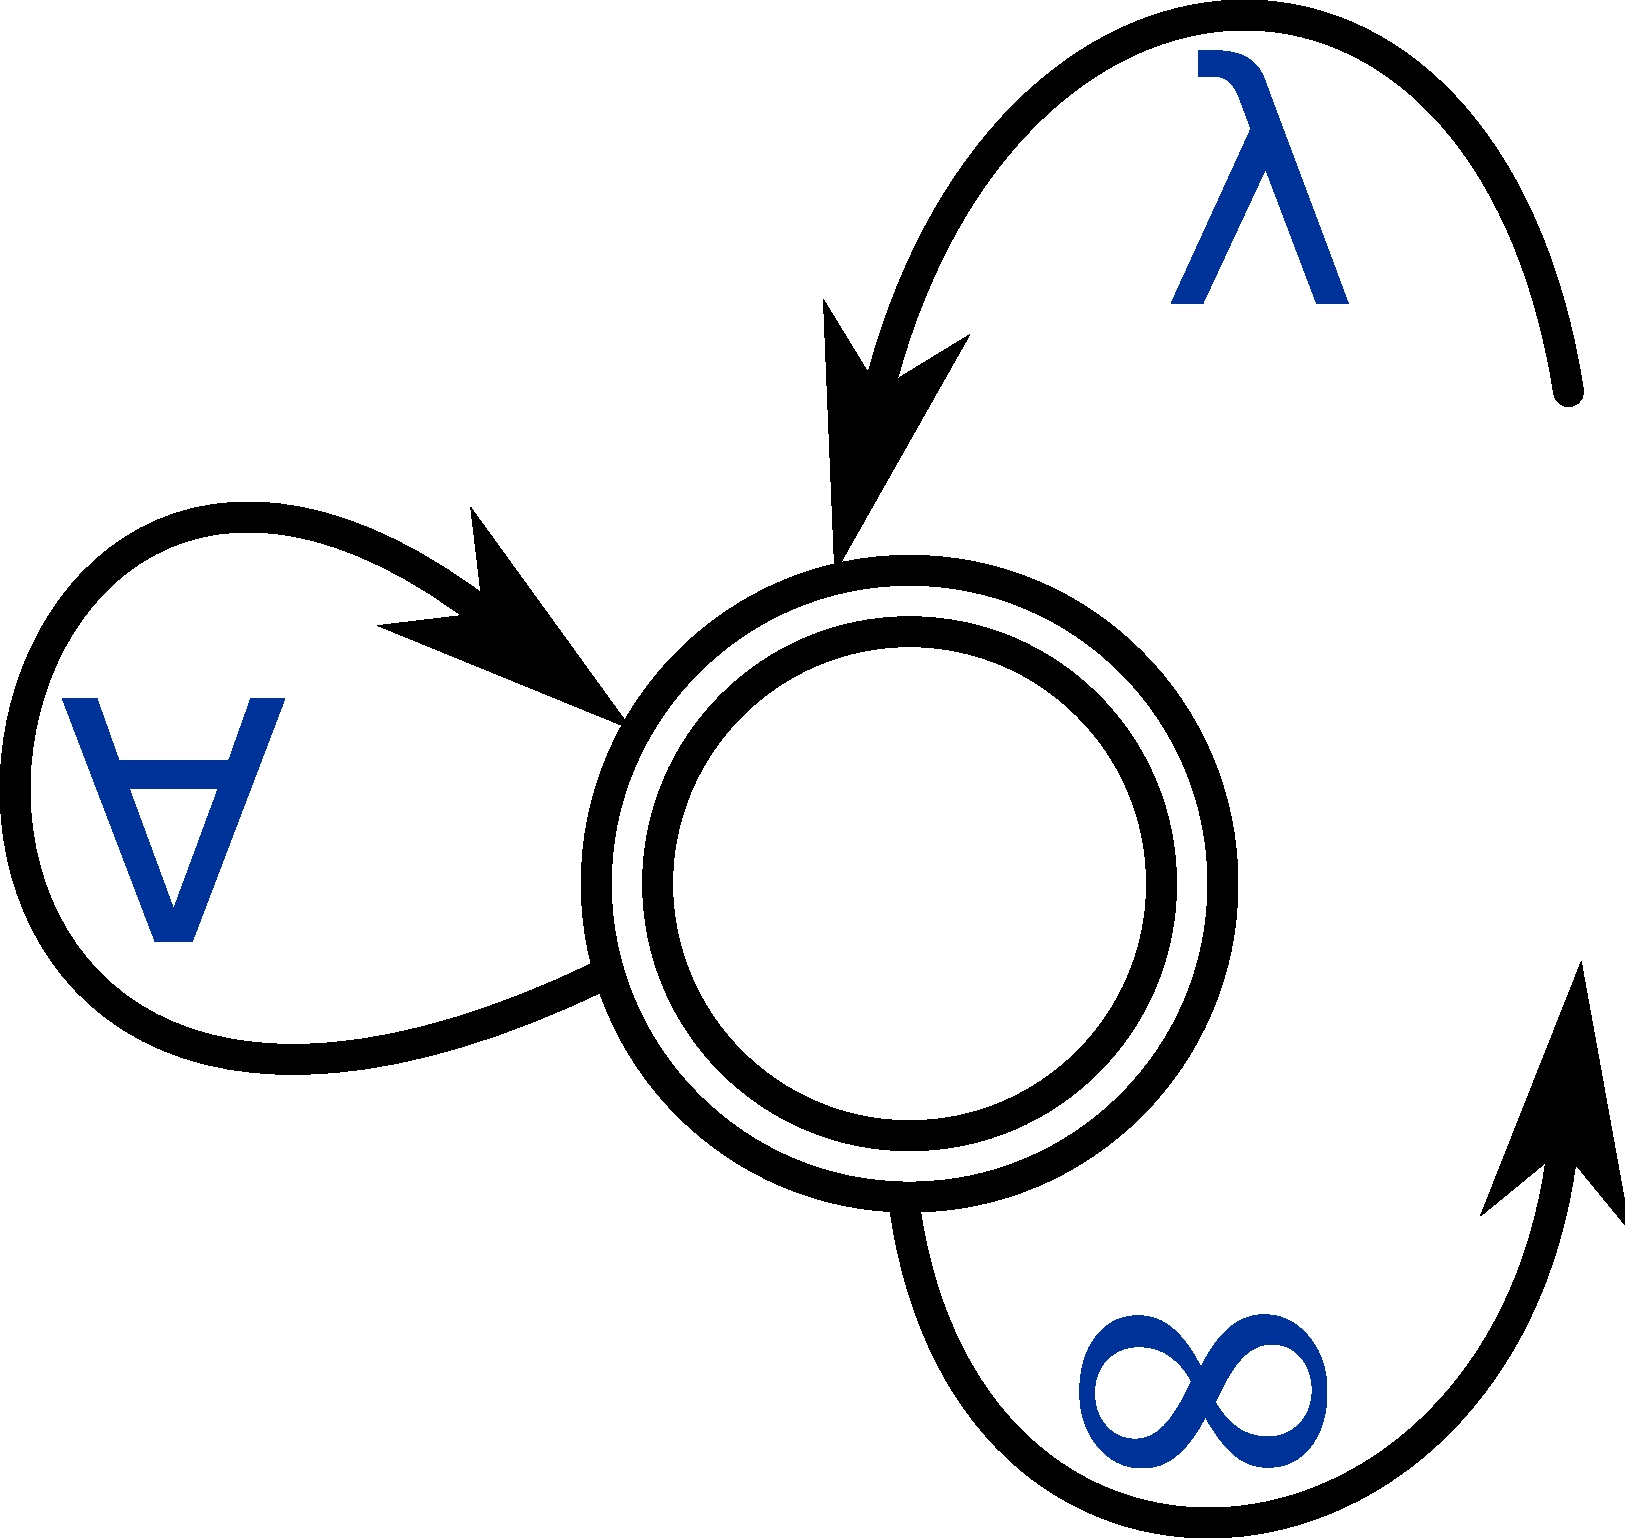
\includegraphics[scale=0.15]{Images/logo.jpg}
	\vspace{2cm}\\
	
	%title
	\Huge \textbf{Argumentation Theory,}\\ \Large \textbf{a gentle Introduction}\\
	\vspace{2cm}
	{\large \textbf{BACHELOR'S THESIS}} \vspace{2.5mm}\\ {\small submitted in partial fulfillment of the requirements for the degree of} \vspace{2.5mm}\\ 
	{\large \textbf{Bachelor of Science}} \vspace{2.5mm}\\ {\small in} \vspace{2.5mm}\\ {\large Software- and Information Engineering} \vspace{2.5mm}\\
	{\small by} \vspace{2.5mm}\\
	%author
	\huge \textbf{Christoph Groß, 1025119}\\
\end{center}
	%advisor
	\vspace{2cm}
\begin{flushleft}
	\begin{adjustwidth}{-0.5in}{}
	{\small to the Faculty of Informatics \\ at the Vienna University of Technology \vspace{2.5mm}\\ Advisor: Ao.Prof.Dipl.-Ing.Dr.techn. Christian Georg Fermüller}
	\end{adjustwidth}
\end{flushleft}

\end{titlepage}
\restoregeometry{}

\begingroup{}
%Table of Contents
\tableofcontents{}

%List of Figures
\listoffigures
\endgroup{}

%Statutory Declaration
\chapter*{Statutory Declaration}
\addcontentsline{toc}{chapter}{Statutory Declaration}

Hereby I assure that this thesis is a result of my personal work and that no other than the indicated aids have been used for its completion.\\
Furthermore I assure that all the quotations and statements, that have been inferred literally or in a general manner from published or unpublished writings, are marked as such.\\
Beyond this I assure that the work has not been used, neither completely nor in parts, to pass any previous examination.

\vspace{1.5cm}
Vienna, \today
\hspace{1.5cm}
\begin{tabular}{l}
\makebox[2.5in]{\hrulefill}\\
Christoph Groß\\
\end{tabular}

%Acknowledgements
\chapter*{Acknowledgements}
\addcontentsline{toc}{chapter}{Acknowledgements}

$D := \mbox{Friends} \cup \mbox{Family} \cup \mbox{University} \cup \{christoph\}$\\
$Friends = \{\text{Max,Pia,Lea,Tobi,Johannes}\}$, \\ $Family = \{\text{Sabine,Gerald,Angelika,Johann,Johanna}\}$, \\ $University = \{\text{Prof.Fermüller}\}$ \\
\[\forall x \in D: (proofread(x) \lor listenToWhining(x) \lor help(x)) \implies thanks(christoph,x)\]

%Abstract
\chapter*{Abstract}
\addcontentsline{toc}{chapter}{Abstract}

This thesis explores the concept of argumentation frameworks in general and particularily in the context of nonmonotonic reasoning.\\
First off, the necessary formal definitions are introduced, a few easy examples are given as clarification and then the theoretical conclusions are drawn.\\
Then, the link between argumentation frameworks and default theory will be shown as an example of how argumentation theory can be used for dealing with nonmonotonic reasoning.\\
In the next step, the reader receives information about things that have not been dealt with in this thesis, some exemplary tools and systems and also
pointers to the needed sources to get a deeper understanding of the subject.\\
Finally, the documentation of an application specifically written during the course of this thesis is appended whith the purpose to graphically help understanding the subject.\\

\raggedright %left-align whole text
%Chapter 1, Introduction
\chapter{Introduction}

%Nonmonotonic reasoning
%\section{Nonmonotonic Reasoning}
%\begin{elab}[Monotonicity]
%If for a given set of formulas $\bm{\psi}$ and a formula $\bm{A}$ the logical consequence $\bm{\psi \vdash A}$ holds,\\ then $\bm{\psi,B \vdash A}$ still holds.
%\end{elab}
%As one can see, nonmonotonic sets of formulas might change their deducable knowledge as new facts are added. 

\section{Argumentation Theory}
In a human context, we (hopefully) argue to reach a sound conclusion. We do that by claiming statements 
based on premisses, and usually, due to different perception of subjects as well as other factors,
these statements tend to vary in their degree of believability.

Argumentation theory in general, is the interdisciplinary study of how conclusions can be reached  through logical reasoning.
Since this is a very wide field, I can not hope to discuss all of it here.\\
 The \href{http://en.wikipedia.org/wiki/Argumentation_theory}{http://en.wikipedia.org/wiki/Argumentation\_theory} article provides a good overview
for interested readers.

This thesis focuses on the logical approach by Dung in his milestone paper from 1995 \cite{Dung},
the so called "argumentation frameworks".
Argumentation Frameworks try to formalize arguments and their semantics.
To this purpose, there are two main components. First, there are arguments modeled as formulas and second, there are attack relations between said arguments.

\subsection{Argumentation Frameworks}
\begin{mydefn}[Argumentation Framework - \cite{Dung}]
An argumentation framework $\bm{AF}$ is defined as a tuple, consisting of a finite set of arguments ($\bm{AR}$) and a 
set of attack relations ($\bm{att}$).\\
Attack relations are tuples of two arguments where the first argument attacks the second one.
$\bm{AF:=\langle AR,att \rangle}$
\end{mydefn}

\begin{myrmrk}
It is also possible for a set of arguments to attack an argument: $\bm{S \text{ attacks } a \text{ iff } \exists a' \in S: a' \text{ attacks } a}$
\end{myrmrk}

The following example shows that an argumentation framework can either be written in a form according to this definition, or visualized as a directed graph.

\newpage

\begin{myexmpl}
$\bm{s=}$"Superman is the best superhero!", $\bm{b=}$"Batman is the best superhero!",\\$\bm{a=}$"Only Aquaman rules over the seas.", $\bm{r=}$"Robin is Batman's sidekick."\\
$\bm{AR = \{a,b,s\}}$, $\bm{att=\{(b,s),(b,a),(a,s),(a,b),(s,b),(s,a),(b,r)\}}$
\label{a b s r}
\end{myexmpl}

\begin{figure}[h!]
\begin{center}\begin{tikzpicture}
	\node[state](a){$a$};
	\node[state](s)[above right=of a]{$s$};
	\node[state](b)[below right=of s]{$b$};
	\node[state](r)[right=of b]{$r$};
	\path[->,thick](s) edge[bend left] (b);
	\path[->,thick](s) edge[bend left] (a);
	\path[->,thick](a) edge[bend left] (b);
	\path[->,thick](a) edge[bend left] (s);
	\path[->,thick](b) edge[bend left] (a);
	\path[->,thick](b) edge[bend left] (s);
	\path[->,thick](b) edge[bend left] (r);
\end{tikzpicture}\end{center}
\caption{graph of AF (example \ref{a b s r})}
\end{figure}

%Properties of argumentation frameworks
\subsection{Properties of (Sets of) Arguments}

The following definitions are originally found in \cite{Dung}.

%basic properties: conflict free, acceptable, admissible
\begin{mydefn}[Conflict-freeness]
A set \textbf{S} of arguments is said to be conflict-free, if for any argument $\bm{a \in S}$, there is no other argument $\bm{b \in S}$ so that $\bm{(a,b) \in att}$.
\end{mydefn}

\begin{mydefn}[Acceptability]
An argument $\bm{a \in AR}$ is acceptable with respect to a set \textbf{S}, iff \textbf{S} attacks each argument $\bm{b \in AR}$ that attacks \textbf{a}. 
\end{mydefn}

\begin{myfrmrk}
If for said argument $\bm{a}$ is not being attacked by any $\bm{b \in AR}$, then it is acceptable even with respect to the empty set.
\end{myfrmrk}

\addcontentsline{toc}{subsection}{Admissible Extensions}
\begin{mydefn}[Admissibility]
A conflict-free set \textbf{S} is said to be admissible, iff each argument $\bm{a \in S}$ is acceptable with respect to \textbf{S}.
Often, \textbf{S} is also called an admissible extension.
\label{admissible}
\end{mydefn}
\begin{myrmrk}
In example \ref{a b s r}, the admissible extensions would be $\bm{E_A = \{\emptyset,\{a\},\{b\},\{s\},\{r,a\},\{r,s\}\}}$. 
\end{myrmrk}

These are the basic properties that can be fulfilled by arguments or sets of arguments. Based on them, we will now introduce a few more interesting definitions.
For instance, argumentation frameworks know a number of different extensions, which can be used to capture the semantics of their subsets. 

\newpage
If not explicitly marked, all the following extensions can also be originally found in \cite{Dung}.

\begin{myrmrk}[\textbf{Notation of extensions}]
From here on, we will use $\bm{E_{i}}$ to denote an arbitrary but fixed extension of type $\bm{i \text{, while } E_{I}}$ denotes the set of all extensions of type $\bm{i}$.\\
\end{myrmrk}

The first of those extensions takes a rather gullible approach to things; the so called \textit{preferred extension} is defined as follows:

\addcontentsline{toc}{subsection}{Preferred Extensions}
\begin{mydefn}[Preferred Extensions]
$\bm{E_{p}}$ is a preferred extension of \textbf{AF}, iff $\bm{E_{p}}$ is a maximal admissible set (with respect to set inclusion) of \textbf{AF}.
\end{mydefn}

\begin{myrmrk}
In example \ref{a b s r}, the preferred extensions would be $\bm{E_{P} = \{\{b\},\{r,a\},\{r,s\}\}}$.
\end{myrmrk}

To avoid any confusions, the alternative definition for preferred extensions in \cite{Egly} can be useful.\\
As it is pointed out there, every admissible set that is not a true subset of any other admissible set, is in fact a preferred extension.\\
The following lemma will be useful later on.
\begin{mylem}[\cite{Dung}]
For every AF, there exists at least one preferred extension.
\end{mylem}

\begin{myprf}
The proof depends on two different properties of admissible sets:
\begin{enumerate}
	\item{The empty set is always admissible.}
	\item{Given an admissible Set $\bm{S}$ and an argument $\bm{\{a\}}$, which is acceptable with respect to $\bm{S \cup \{a\}}$, the unification $\bm{S \cup a}$ is also admissible.}
\end{enumerate}
$(1)$ directly follows from the definition \ref{admissible}\\
$(2)$ We just have to show, that $\bm{S \cup \{a\}}$ is conflict-free. To achieve that, we assume the contrary:\\ 
There exists an argument $\bm{b \in S \text{ so that either } (a,b) \text{ or } (b,a)}$ holds.
There has to be an argument $\bm{c \in S}$, so that either $\bm{(c,a) \text{ or } (c,b) \text{. We know, that } S \text{ is conflict-free, so } (c,b) \implies \text{\Lightning}}$\\
On the other hand, $\bm{c \text{ and } a}$ are both acceptable with respect to $\bm{S \text{; } (c,a) \implies \text{\Lightning}}$.  
\end{myprf}

Another approach would be the \textit{stable extension}, which is defined as follows:

\newpage

\addcontentsline{toc}{subsection}{Stable Extensions}
\begin{mydefn}[Stable Extensions]
The conflict-free set $\bm{E_{s}}$ is a stable extension of \textbf{AF}, iff $\bm{E_{s}}$ attacks each argument $\bm{a \notin E_{s}}$.
\end{mydefn}

\begin{myrmrk}
In example \ref{a b s r}, the stable extensions would be $\bm{E_{S} = \{\{b\},\{r,a\},\{r,s\}\}}$.
\end{myrmrk}

\addcontentsline{toc}{subsection}{Complete Extensions}
\begin{mydefn}[Complete Extensions]
The admissible set $\bm{E_{c}}$ is a complete extension of \textbf{AF} iff every argument which is acceptable with respect to $\bm{E_{c}}$ is included in $\bm{E_{c}}$.
\end{mydefn}

\begin{myrmrk}
In example \ref{a b s r}, the complete extensions would be $\bm{E_{C} = \{\emptyset,\{b\},\{r,a\},\{r,s\}\}}$.
\end{myrmrk}

It is easy to see that many different complete extensions can exist. That leads directly to the \textit{grounded extension}.

\addcontentsline{toc}{subsection}{Grounded Extensions}
\begin{mydefn}[Grounded Extensions - \cite{Egly}]
The intersection of all complete extensions $\bm{S_{i} \text{ for } i \in \{1..n\}}$, is called the grounded 
extension.\\ $\bm{E_{g} := \bigcap\limits^{n}_{i=1}{S_{i}}}$
\label{ground ext}
\end{mydefn}

\begin{myrmrk}
In example \ref{a b s r}, the only grounded extension would be $\bm{E_{g} = \emptyset}$.
\end{myrmrk}

\addcontentsline{toc}{subsection}{Semi-stable Extension}
\begin{mydefn}[Semi-stable Extensions - \cite{Caminada}]
A set $\bm{E_{ss}}$ is a semi-stable extension, if it is a complete extension and the set $\bm{E_{ss} \cup \{a \in AR \vert E_{ss} \text{ attacks }a\}}$
is maximal (with respect to set inclusion).
\label{semi ext}
\end{mydefn}

\newpage

\begin{myexmpl}
The following example from \cite{Caminada} illustrates that not every semi-stable extension is also stable.\\
In the following graph, the set $\bm{E_{ss}=\{b,d\}}$ is semi-stable but not stable\\(because $\bm{a}$ is not attacked by $\bm{E_{ss}}$).
\label{stable != semi-stable}
\end{myexmpl}
\begin{figure}[h!]
\begin{center}\begin{tikzpicture}
	\node[state](c){$c$};
	\node[state](a)[above left = of c]{$a$};
	\node[state](b)[below left = of c]{$b$};
	\node[state](d)[right = of c]{$d$};
	\path[->,thick](a) edge[loop left] (a);
	\path[->,thick](a) edge (c);
	\path[->,thick](b) edge (c);
	\path[->,thick](c) edge (d);
\end{tikzpicture}\end{center}
\caption{semi-stable but not stable (example \ref{stable != semi-stable})}
\end{figure}

\addcontentsline{toc}{subsection}{Ideal Extension}
\begin{mydefn}[Ideal Extensions - \cite{Dung2}]
A set $\bm{E_{i}}$ is the ideal extension, if it is a maximal admissible set, that is contained in every preferred extension.
\label{ideal ext}
\end{mydefn}

\begin{myexmpl}
The following example illustrates ideal extensions (and how they differ from e.g. grounded extensions).\\
In the following graph, the set $\bm{E_{I}=\{\{b\}\}}$ contains the only ideal extension.
As we can see, $\bm{E_{i}}$ is a subset of every preferred extension ($\bm{\{b,c,f\},\{b,d,f\}}$).
This example can also be found in \cite{Dung2}.

\label{ideal extension}
\end{myexmpl}
\begin{figure}[h!]
\begin{center}\begin{tikzpicture}
	\node[state](a){$a$};
	\node[state](b)[right = of a]{$b$};
	\node[state](c)[above right = of b]{$c$};
	\node[state](d)[below right = of b]{$d$};
	\node[state](e)[below right = of c]{$e$};
	\node[state](f)[right = of e]{$f$};
	\path[->,thick](a) edge[loop left] (a);
	\path[->,thick](a) edge[bend left] (b);
	\path[->,thick](b) edge[bend left] (a);
	\path[->,thick](c) edge[bend left] (d);
	\path[->,thick](d) edge[bend left] (c);
	\path[->,thick](c) edge (e);
	\path[->,thick](d) edge (e);
	\path[->,thick](e) edge (f);
\end{tikzpicture}\end{center}
\caption{ideal extension (example \ref{ideal extension})}
\end{figure}


\newpage

\subsection{Examples of different Extensions}
Contrary to the previous section, where different aspects of one example were used to accompany the definitions of extensions, 
here I am going to provide examples which simply are interesting in their respective results.

\begin{myexmpl}
$\bm{s_{1}=}$"Superman is the best superhero!", $\bm{b_{1}=}$"Batman is way cooler..",\\
$\bm{s_{2}=}$"But Superman is stronger.", $\bm{b_{2}=}$"Batman possesses genius-level intellect."\\
$\bm{AR = \{s_{1},s_{2},b_{1},b_{2}\}}$, $\bm{att = \{(b_{1},s_{1}),(s_{2},b_{1}),(b_{2},s_{2})\}}$
\label{s1 s2 b1 b2 ex}
\end{myexmpl}

This argumentation framework could also be depicted by following graph.

\begin{figure}[h!]
\begin{center}\begin{tikzpicture}
	\node[state](s1){$s_{1}$};
	\node[state](b1)[right=of s1]{$b_{1}$};
	\node[state](s2)[right=of b1]{$s_{2}$};
	\node[state](b2)[right=of s2]{$b_{2}$};
	\path[->,thick] (b2) edge (s2);
	\path[->,thick] (s2) edge (b1);
	\path[->,thick] (b1) edge (s1);
\end{tikzpicture}\end{center}
\caption{graph of AF (example \ref{s1 s2 b1 b2 ex})}
\end{figure}

The extensions of this example would be 
\begin{itemize}
	\item{$\bm{E_{P}=E_{S}=E_{C}=E_{G}=\{\{b_{1},b_{2}\}\}}$}
\end{itemize}

The next example is going to be a little more interesting in its outcome.
\begin{myexmpl}
$\bm{s1=}$"Superman was born a hero.", $\bm{s2=}$"Superman trained hard to become a hero."\\
$\bm{AR=\{s1,s2\}}$, $\bm{att=\{(s1,s2),(s2,s1)\}}$
\label{s1 s2 ex}
\end{myexmpl}

This examples graph looks like this.
\begin{figure}[h!]
\begin{center}\begin{tikzpicture}
	\node[state](s1){$s1$};
	\node[state](s2)[right=of s1]{$s2$};
	\path[->,thick](s1) edge[bend left] (s2);
	\path[->,thick](s2) edge[bend left] (s1);
\end{tikzpicture}\end{center}
\caption{graph of AF (example \ref{s1 s2 ex})}
\end{figure}

Following extensions can be calculated
\begin{itemize}
	\item{$\bm{E_{P}=E_{S}=\{\{s1\},\{s2\}\}}$}
	\item{$\bm{E_{C}=\{\emptyset,\{s1\},\{s2\}\}}$}
	\item{$\bm{E_{G}=\{\emptyset\}}$}
\end{itemize}

\newpage

\begin{myexmpl}
$\bm{b=}$"The superhero Batman is human. No humans are superheros."\\
$\bm{AR=\{b\}}$, $\bm{att=\{(b,b)\}}$
\label{b loop ex}
\end{myexmpl}

The corresponding graph looks like follows.
\begin{figure}[h!]
\begin{center}\begin{tikzpicture}
	\node[state](b){$b$};
	\path[->,thick](b) edge[loop left] (b);
\end{tikzpicture}\end{center}
\caption{graph of AF (example \ref{b loop ex})}
\end{figure}

For this example, the extensions would look as follows.
\begin{itemize}
	\item{$\bm{E_{p}=E_{c}=E_{g}=E_{s}=\emptyset}$}
\end{itemize}

\newpage

\begin{myexmpl}
Last but not least, we are going to take a look on a slightly more complex example, that gives a deeper insight
in the relations between the extensions. It should be considered along with \textbf{Figure \ref{hierarchy graph}}.\\
In the graph below, following different extensions can be ovserved:
\begin{itemize}
	\item{semi-stable extension $\bm{E_{ss}=\{d,e\}}$}
	\item{preferred extensions $\bm{E_{P}=\{\{b,c\},\{d,e\}\}}$}
	\item{complete extensions $\bm{E_{C}=\{\{b,c\},\{d,e\},\{j\}\}}$}
	\item{grounded extension $\bm{E_{g}=\emptyset}$}
	\item{ideal extension $\bm{E_{i}=\emptyset}$}
\end{itemize}
\label{relations of extensions}
\end{myexmpl}
\begin{figure}[h!]
\begin{center}\begin{tikzpicture}
	\node[state](a){$a$};
	\node[state](b)[above right = of a]{$b$};
	\node[state](c)[below right = of a]{$c$};
	\node[state](d)[right = of b]{$d$};
	\node[state](e)[right = of c]{$e$};
	\node[state](f)[above right = of d]{$f$};
	\node[state](g)[right = of d]{$g$};
	\node[state](h)[right = of e]{$h$};
	\node[state](i)[below right = of e]{$i$};
	\node[state](j)[above right = of b,above left = of d]{$j$};
	\path[->,thick](a) edge[loop left] (a);
	\path[->,thick](f) edge[loop right] (f);
	\path[->,thick](g) edge[loop right] (g);
	\path[->,thick](h) edge[loop right] (h);
	\path[->,thick](i) edge[loop right] (i);
	\path[->,thick](a) edge[bend left] (b);
	\path[->,thick](b) edge[bend left] (a);
	\path[->,thick](a) edge (c);
	\path[->,thick](b) edge[bend left] (d);
	\path[->,thick](b) edge[bend left] (e);
	\path[->,thick](d) edge[bend left] (b);
	\path[->,thick](e) edge[bend left] (b);
	\path[->,thick](d) edge (f);
	\path[->,thick](d) edge (g);
	\path[->,thick](d) edge (h);
	\path[->,thick](d) edge (i);
	\path[->,thick](e) edge (f);
	\path[->,thick](e) edge (g);
	\path[->,thick](e) edge (h);
	\path[->,thick](e) edge (i);
	\path[->,thick](b) edge (j);
	\path[->,thick](j) edge (b);
	\path[->,thick](d) edge (j);
	\path[->,thick](j) edge (d);
	\path[->,thick](e) edge (j);
	\path[->,thick](j) edge (e);
\end{tikzpicture}\end{center}
\caption{relations of extensions (example \ref{relations of extensions})}
\end{figure}

\medskip
\begin{myrmrk}
Now it comes to attention that there are no stable and semi-stable extensions in the above example at the same time.
That is because it is not possible for distinctive stable and semi-stable extensions to coexist in a single AF. 
We will take a quick look at the reasons for this particular relation.
\end{myrmrk}
\begin{myprf}
Assume the contrary, i.e. there exists a stable extension $\bm{E_{s}}$ and a (only) semi-stable extension $\bm{E_{ss}}$.
From the definitions of stable and semi-stable extensions follows\\
$\bm{E_{s} \cup \{a \vert E_{s} \text{ attacks } a\} = AR}$. Since every semi-stable extension has to fulfill 
$\bm{E_{ss} \cup \{a \vert E_{ss} \text{ attacks } a\} \textbf{ is maximal with respect to set inclusion}}$,
it is clear that $\bm{E_{ss}}$ has to attack every argument outside of itself, in order to achieve maximum set inclusion.\\
This directly contradicts the assumption $\bm{E_{s} \notin \{E \vert \text{ E is a stable extension }\} \implies \text{\Lightning}}$.
\end{myprf}

\chapter{Conclusions and Implications}

Now that we have established the necessary definitions, it is time to travel further down the rabbit hole and explore the meaning of what we just defined.

\section{Relations between different Extensions}
The following, simple tree graph (borrowed from \cite{Hunter}) shows the hierarchy of extension types better than words could ever describe it.
\begin{figure}[h!]
\begin{center}\begin{tikzpicture}[node distance=0.5cm, auto,
	mynode/.style={rectangle,draw=black}]
	\node[mynode] (stable) {stable};
	\node[mynode] (semi-stable) [above right = of stable] {semi-stable};
	\node[mynode] (preferred) [above right = of semi-stable] {preferred};
	\node[mynode] (complete) [above right = of preferred] {complete};
	\node[mynode] (grounded) [below = of complete] {grounded};
	\node[mynode] (ideal) [below right = of complete] {ideal};
	\node[mynode] (admissible) [above right = of complete] {admissible};
	\path[->] (stable) edge (semi-stable);
	\path[->] (semi-stable) edge (preferred);
	\path[->] (preferred) edge (complete);
	\path[->] (grounded) edge (complete);
	\path[->] (ideal) edge (complete);
	\path[->] (complete) edge (admissible);
\end{tikzpicture}\end{center}
\caption[hierarchy of extension types]{hierarchy of extension types - 
	An arrow from X to Y denotes that an X-extension is also a Y-extension.}
\label{hierarchy graph}
\end{figure}

\newpage

Now I want to show a few specific relations between those aforementioned extensions, since they will be reused in later proofs.

\begin{mylem}[\cite{Dung}]
%latex interprets the first item of the list as a sentence, therefore this "bogus" first sentence.
\leavevmode\vspace{-\baselineskip}
\begin{enumerate}
	\item{Every preferred extension is a complete extension, but not vice versa.}
	\item{The grounded extension is the least (with respect to set inclusion) complete extension}
\end{enumerate}
\end{mylem}

\begin{myprf}[1]
It is obvious that every preferred extension (maximum admissible set) is a complete extension.\\
Let $\bm{AR=\{a,b\}}$ and $\bm{att=\{(a,b),(b,a)\}}$.\\
Then it is easy to see, that $\bm{E_{P}=\{\{a\},\{b\}\}}$ but $\bm{E_{C}=\{\emptyset,\{a\},\{b\}\}}$\\
$\bm{\implies \exists E_{c}: E_{c} \in E_{C} \land E_{c} \notin E_{P} \implies \text{\Lightning}}$
\end{myprf}

\begin{myprf}[2]
Proof for this lemma follows directly from definition \ref{ground ext}.
\end{myprf}

\newpage

\section{Properties of Argumentation Frameworks}
Up to now, we have only talked about sets of arguments and their properties. Now we will focus on the whole argumentation framework and 
make a connection between its properties and extensions.

\subsection{Well-Founded Argumentation Frameworks}
The first new property establishes a coherence between preferred, grounded and stable extensions.
\begin{mydefn}[\cite{Dung}]
An argumentation framework is called well-founded, iff there exists no infinite sequence of arguments $A_{0},A_{1},\dots,A_{n},\dots$ where each $A_{i+1}$ attacks $A_{i}$.
\end{mydefn}

\begin{myfrmrk}
This infinite sequence of arguments can be formed by a finite set of arguments (for instance $AR=\{a,b\}$, $att={\{(a,b),(b,a)\}}$).
\end{myfrmrk}

Following lemma can be extracted from this definition.
\begin{mylem}[\cite{Dung}]
Every well-founded AF has exactly one complete extension, which is also a preferred, grounded and stable extension.
\end{mylem}

\begin{myprf}
Assumption: $\bm{\text{AF is well-founded and } E_{g} \text{ is not stable}}$.
We further assume, that $\bm{\exists a \in AR \text{\textbackslash} E_{g} \text{ and } \nexists b \in E_{g}:(b,a) \in att}$.\\
\bigskip
If $\bm{a}$ is not acceptable with respect to $\bm{E_{g}}$, this means that there has to be another argument $\bm{c \in AR \text{\textbackslash} E_{g}}$, 
which is also not attacked by $\bm{E_{g}}$. \\ Therefore an infinite sequence of arguments like $\bm{a \text{ and }c}$ has to exist $\implies \text{\Lightning}$.
\end{myprf}

% --- Coherent Argumentation Frameworks ---
%\subsection{Coherent Argumentation Frameworks}
%If an AF has a preferred extension, which is not a stable one too, that indicates some sort of "anomaly" in the framework (see example \ref{b loop ex}).\\
%So what we want to do next, is to find out what criteria has to be met so that preferred and stable extension coincide.

%\begin{mydefn}[\cite{Dung}]
%An AF is called coherent, if $\bm{E_{P} = E_{S}}$.
%\end{mydefn}

%\begin{myrmrk}
%It follows directly from the definition, that there always exists at least one stable extension in a coherent AF.
%\end{myrmrk}

\chapter{Argumentation Theory and Nonmonotonic Reasoning}

One reason why argumentation frameworks are important and useful is the fact that they can easily be used to model other
logical constructs, often making working with those less complex.\\
For instance, the nonmonotonic "Default Logic", which is briefly described in the following section.
Since all the definitions in this next section were taken from \cite{Reiter}, that paper provides more insight to the interested reader.

\section{Default Logic}
In classical logic, it is not possible to conclude new knowledge from uncertain/unknown information. One scenario for instance, would be the modeling of a default property,
which could be assigned to any object as long as we do not have any contradicting facts.\\
This is where default logic comes in handy.

\begin{mydefn}[Default Logic]
A default theory is a pair $\bm{\langle W,D \rangle}$.
$\bm{W}$ is the knowledge base, consisting of logical formulas, $\bm{D}$ is a set of \textit{default rules}.
Each default rule has following form: \[\bm{\frac{Prerequisite : Justification_{1},\dots,Justification_{n}}{Conclusion}}\]
\end{mydefn}

A simple (and maybe overused) example is the following.
\begin{myexmpl}
\[\bm{D = \frac{Bird(tweety): Flies(Tweety)}{Flies(Tweety)}}\]
$\bm{W_{1} = \{Bird(tweety)\}}$
$\bm{W_{2} = \{Bird(tweety),Penguin(tweety),Penguin(X) \implies \lnot Flies(X)\}}$
\end{myexmpl}
As we can see, as long as no facts, that negate one of the justifications, can be deduced from our knowledge base, we can infere the conclusion that Tweety can fly
(which would be the case with $\bm{W_{1}}$).\\
On the other hand (with $\bm{W_{2}}$), we could deduce $\bm{\lnot Flies(Tweety)}$, therefore the Justifications would not be met and the default would be overruled by
the more important fact.

Furthermore we have to define the so-called "Reiter's extension" (or R-extension).
\begin{mydefn}
A R-extension of a default theory $\bm{\langle W,D \rangle}$ is a set of formulas $\bm{E_{R}}$, that satisfies following conditions:
\begin{itemize}
	\item{$\bm{E_{R} = \bigcup \{W_{i} \vert i \text{ is a natural number}\}}$}
	\item{$\bm{W_{0} = W}$}
	\item{$\bm{W_{i+1} = Th(W_{i}) \cup \{w \vert \exists(p:j_{1},\text{\dots},j_{k}/w) \text{ in } D \text{ so that } \{j_{n}\} \cup E \text{ consistent for } k \geq n \geq 1,
		\text{ and } p \in W_{i}\}}$}
\end{itemize}
$Th(T)$ denotes the first order closure of a theory $T$.
\end{mydefn}

\section{Default Logic \& Argumentation Frameworks}
As it is pointed out in 3.1 of \cite{Dung}, a default theory $\bm{T = \langle W,D \rangle}$ can be interpreted as an argumentation framework $\bm{AF_{d} = \langle AR,Att \rangle}$.\\
From here on out, we let $\bm{just(D)}$ denote the set of justifications of a default theory.

The following two criteria are necessary to build the interpretation:
\begin{itemize}
	\item{$\bm{AF_{d} = \{(K,k) \vert K \subseteq just(D)\}}$, so that $\bm{K}$ is a support of the well-formed, closed formula $\bm{k}$ with respect to $\bm{T}$}
	\item{$\bm{(K,k)}$ attacks $\bm{(K',k')}$ iff $\bm{\lnot k \in K'}$}
\end{itemize}

The following lemma shows that this interpretation is not just a coincidence.

\begin{mylem}[\cite{Dung}]
Let $\bm{E_{a}}$ be an admissible subset of $\bm{AF_{d} \text{ and } H = \bigcup \{K \vert (K,k) \in E_{a}\}}$.
Then $\bm{T,H}$ holds, iff $\bm{T}$ is consistent.
\end{mylem}

\begin{myprf}
From left to right, this should be obvious, so we are only going to take a look at the second part of the proof.
To achieve this, we assume the contrary:\\There exists a subset $\bm{K \text{ of } H \text{, so that } T,K \vdash \bot}$.
Thus, for every $\bm{k \text{, }(K,k) \in AR}$. Also, let $\bm{(K',k') \in E_{a}}$ so that $\bm{K'}$ is not empty.
Now $\bm{(K,k)}$ represents an attack on $\bm{(K',k')}$.\\Given the admissibility of $\bm{E_{a}}$, there has to be some argument $\bm{a = (H',h') \in E_{a}}$, so that
$\bm{\lnot h' \in K}$; in other words, since $\bm{(K,k),(K',k') \in E_{a}}$ and the admissibility of $\bm{E_{a} \text{, the set cant be conflict-free} \implies \text{\Lightning}}$ 
\end{myprf}

\newpage

Now that we have established the possibility to interprete default theories as argumentation frameworks, we want to examine this relationship more closely.
There is a correspondence between the R-extensions of a default theory and the stable extensions of an argumentation framework.\\
To show this, we need some more definitions:

\begin{mydefn}[\cite{Dung}]
Let $\bm{S}$ be a first order theory and $\bm{S'}$ be a set of arguments of $\bm{AF_{d}}$. Then, we define:\\
\begin{itemize}
	\item{$arg(S) = \{(K,k) \in AR \vert \forall j \in K: \{j\} \cup S \text{ is consistent}\}$}
	\item{$flat(S') = \{k \vert \exists(K,k) \in S'\}$}
\end{itemize}
\end{mydefn}

Together with the definition of the R-extension, the following lemmata become obvious:\\
\begin{mylem}[\cite{Dung}]
If $\bm{T}$ is a default theory and $\bm{E}$ is a first order theory. Then, $\bm{E}$ is a R-extension of $\bm{T}$ iff $\bm{E = flat(arg(E))}$.
\end{mylem}

\begin{mylem}[\cite{Dung}]
$\bm{T = \langle W,D \rangle}$ be a default theory, $\bm{E}$ a R-extension of $\bm{T}$ and $\bm{E'}$ a stable extension of $\bm{AF_{d}}$.
Then \\
\begin{enumerate}
	\item{$\bm{arg(E)}$ is a stable extension of $\bm{AF_{d}}$}
	\item{$\bm{flat(E')}$ is a R-extension of $\bm{T}$}
\end{enumerate}
\end{mylem}

Apparently, the preferred extension semantics of $\bm{AF_{d}}$ generalizes the R-extension semantics of $\bm{T}$.
Also it captures the intuitive idea of default logic more naturally and thus makes it a bit easier to model and understand.
This was just one of the many applications of argumentation frameworks, the interested reader could either get more examples in \cite{Dung} or
head on to the "Further Topics" chapter for more information.

\chapter{Further Topics}
At this point, some attentive reader might notice that we have been dealing with the abstract concept of argumentation frameworks almost exclusively.
Since this is a bachelor's thesis, I had to focus on this one single aspect in order to not get lost in the process of writing it.\\
Therefore, the idea of this fourth chapter is providing you with pointers to related subjects, sources of deeper understanding and real-life applications to tamper with.

\section{Structure and Extraction of Arguments}
Two very interesting topics are the structure of arguments and how they are extracted. During this paper, we only used arguments as abstract objects with no underlying structure.
If we were trying to solve real world problems by implementing them as an argumentation framework, these two things would be necessary though.\\
The general structure of arguments can be described as it is done in the very good wikipedia article 
(\href{http://en.wikipedia.org/wiki/Argumentation_theory#Internal_structure_of_arguments}{http://en.wikipedia.org/wiki/Argumentation\_theory\#Internal\_structure\_of\_arguments}) 
article:\\
\medskip
arguments typically consist of
\begin{itemize}
	\item{a set of assumptions, often called premises or support}
	\item{a conclusion, often called claim}
\end{itemize}
To gain more insight on the structure of arguments, one could also read \cite{HunterBesnard} or \cite{Prakken}.\\
If the reader is more interested in how arguments are extracted from knowledge, a process which ideally follows certain rules, then \cite{Pollock} could be a good source.

\newpage 

\section{Tools \& Systems}
Since we have already established, that argumentation frameworks can be used to model other logical constructs, it is clear that they can also be a useful tool in various proofs.\\
This is, of course, of very little use in the daily life of a software engineer. In general, the areas where logical applications shine, are for instance \textbf{planning},
\textbf{scheduling} or \textbf{software verification}, all areas with a high potential to save some company a lot of money.\\
If one would like to gain more knowledge on these topics, I would like to point him towards the respective \href{http://en.wikipedia.org/}{wikipedia} articles as a starting point.\\
\medskip
There also exist various tools, systems and software implementations based on Dungs argumentation framework. Referring to the last chapter, we note that most of those systems
deal with the structure of arguments and how to extract them.\\
One typical field of usage would be the modelling and (automated) checking of legal arguments in law.
The following list is not complete of course, I merely tried to sum up a few representative examples.
\medskip
\begin{itemize}
	\item{\textbf{ASPIC} - Argumentation Service Platform with Integrated Components}
	\begin{itemize}
		\item{based on Dungs argumentation frameworks}
		\item{introduced in \cite{ASPIC}}
	\end{itemize}
	\item{\textbf{ASPIC+} - Generalized ASPIC}
	\begin{itemize}
		\item{introduced by H.Prakken in \cite{ASPIC+}}
	\end{itemize}
	\item{\textbf{Carneades} - web-based system for argumentation}
	\begin{itemize}
		\item{\href{https://carneades.github.io/}{Carneades github} or \href{https://carneades.github.io/Publications/}{Carneades publications}}
	\end{itemize}
	\item{\textbf{TOAST} - online ASPIC+ implementation}
	\begin{itemize}
		\item{\href{http://toast.arg-tech.org/snaith-reed-comma12.pdf}{ARG-tech: TOAST}}
	\end{itemize}
	\item{\textbf{AIFdb} - database system allowing the storage of argument structures}
	\begin{itemize}
		\item{\href{http://www.arg-tech.org/index.php/projects/aifbdb-user-guide/}{ARG-tech: AIFdb}}
	\end{itemize}
	\item{\textbf{OVA} - Online Visualisation of Argument}
	\begin{itemize}
		\item{\href{http://www.arg-tech.org/index.php/projects/ova}{ARG-tech: OVA}}
	\end{itemize}
\end{itemize}
\medskip
An interesting source that should be mentioned is the \textit{\textbf{COMMA} - Computational Models of Argument} Conference. Most of the above systems are listed amongst
many more topics on the \href{www.comma-conf.org}{COMMA website}.

\chapter{Documentation - KAFFEE}

As mentioned in the abstract, a software tool was written to accompany the reader through this paper and provide the necessary environment to playfully learn more about
the several extensions and their relationships.\\

The source code as well as an executable jar file can be found on \href{https://github.com/e1025119/thesis}{https://github.com/e1025119/thesis}.
Should any questions or ideas for improvement arise, do not hesitate to write to \href{mailto:e1025119@student.tuwien.ac.at}{e1025119@student.tuwien.ac.at}

The \textbf{K}AFFEE \textbf{A}rgumentation \textbf{F}ramework \textbf{F}or \textbf{E}ngineers and \textbf{E}nthusiasts offers following functions:
\begin{itemize}
	\item{Defining new argumentation frameworks}
	\item{Import prepared examples}
	\item{Select different types of extensions}
	\item{Visualize whole AFs as well as subsets}
	\item{Step-by-Step function that explains how an admissible set is created}
\end{itemize}

\bigskip
The general idea of how to use \textbf{KAFFEE} is simple. The tool is made up of three tabs, which are sequentially dependant on the one before, as shown in the following graph.
\bigskip

\begin{figure}[h!]
\begin{center}\begin{tikzpicture}[node distance=1cm, auto,
	mynode/.style={rectangle,draw=black}]
	\node[mynode] (AFTab) {\textbf{Tab "Argumentation Framework"}};
	\node[mynode] (EXTab) [right = of AFTab] {\textbf{Tab "Extensions"}};
	\node[mynode] (STSTab) [right = of EXTab] {\textbf{Tab "Step By Step"}};
	\path[->] (AFTab) edge (EXTab);
	\path[->] (EXTab) edge (STSTab);
\end{tikzpicture}\end{center}
\caption{Workflow in KAFFEE}
\end{figure}

\bigskip
That requires the user to work in tab \#1 first, the "Argumentation Framework" tab.\\Here, the user has to create/import an argumentation framework.\\
Creating a framework can be achieved by submitting arguments and (optional) attack relations. To do so, the user first has to enter a reference name and text (in case of an argument)
or two existing arguments (in case of an attack relation) and then click the corresponding submit button.\\
The faster way is to import one of the existing example frameworks. This can be easily done, the user only has to click \textbf{Examples} in the menu bar and choose one of the provided
examples.

\bigskip
\begin{figure}[h!]
	\begin{center}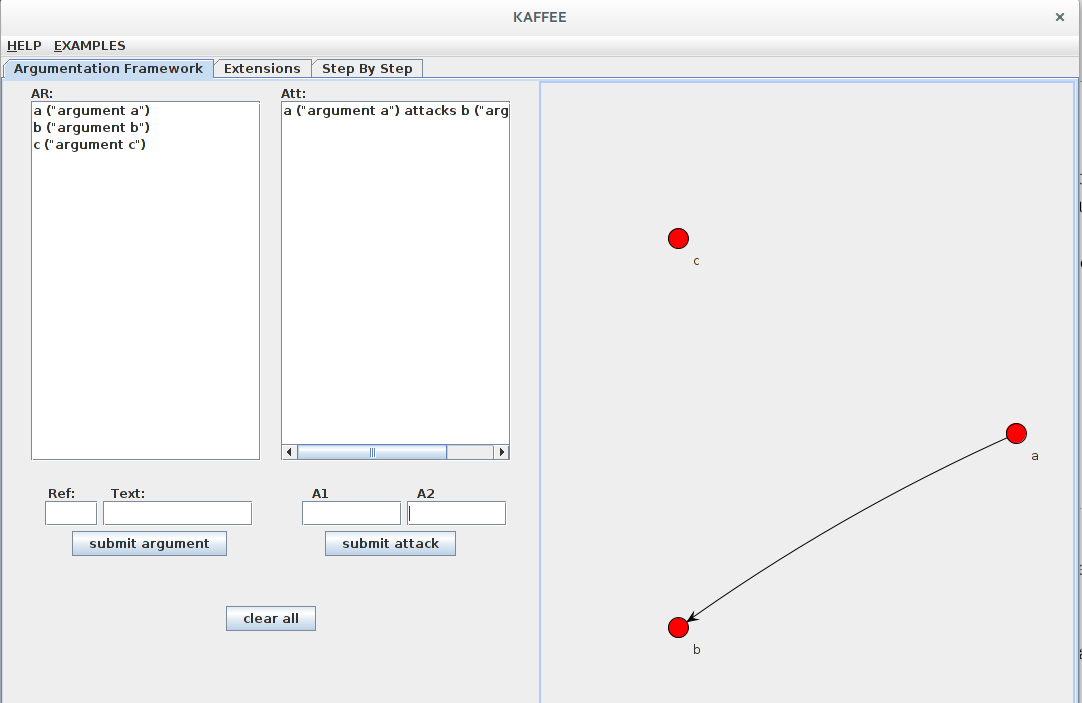
\includegraphics[scale=0.35]{Images/Screenshot_KAFFEE_Tab1.png}
	\end{center}
\caption{Tab "Argumentation Framework"}
\end{figure}

\newpage

Once that is done, the user can either have a look at the visual representation of his/her framework, or continue and switch to the "Extensions" tab.
In this tab, one can choose from a list of possible extensions to be calculated for the given AF. This time, the visual representation on the right will
provide coloring of the selected subset, depending on the chosen extension.\\

\bigskip
\begin{figure}[h!]
	\begin{center}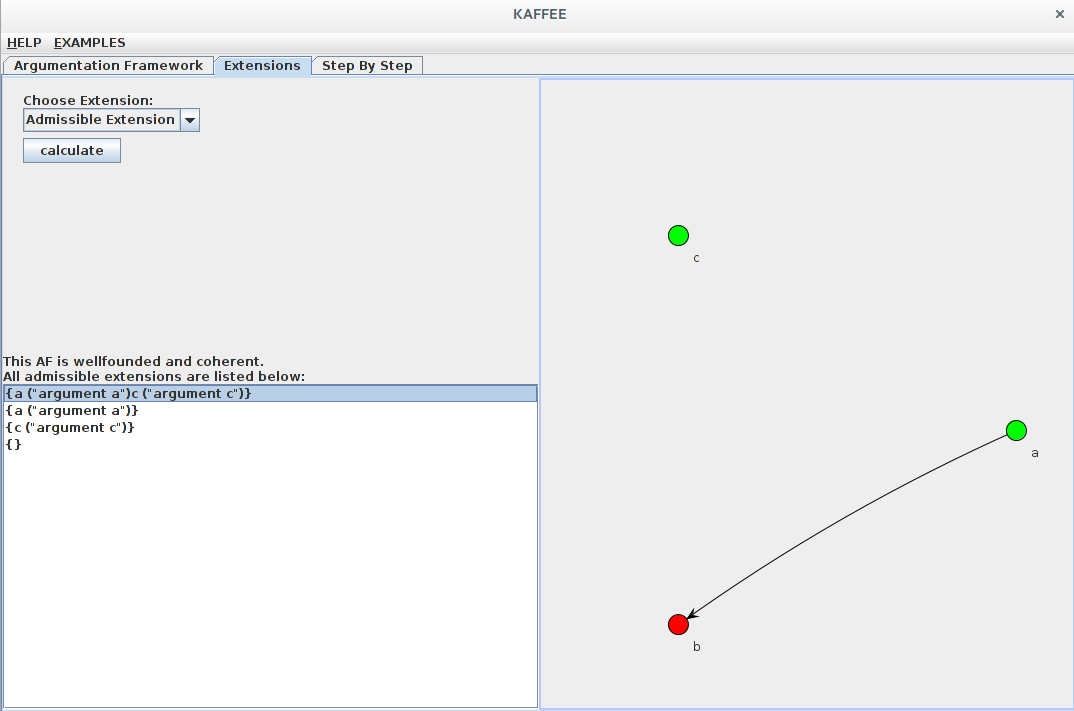
\includegraphics[scale=0.35]{Images/Screenshot_KAFFEE_Tab2.png}
	\end{center}
\caption{Tab "Extensions"}
\end{figure}

\newpage

The last (and optional) tab is the "Step By Step" tab. Here, one can get a better explanation, in a walkthrough kind of style, of how admissible sets are created.\\
In the field "select arguments", the user can choose between going through all elements of the extension, or specific ones to save time.\\
The color coding is as follows:
\begin{itemize}
	\item{\textcolor{red}{red}: the argument is neither part of the extension, nor attacking the argument in question.}
	\item{\textcolor{green}{green}: the argument is part of the extension but currently not active.}
	\item{\textcolor{blue}{blue}: the argument is part of the extension and currently being defended.}
	\item{\textcolor{yellow}{beige}: the argument is attacking the argument currently in question.}
	\item{\textcolor{cyan}{cyan}: the argument is defending the argument currently in question.}
\end{itemize}
 
\bigskip
\begin{figure}[h!]
	\begin{center}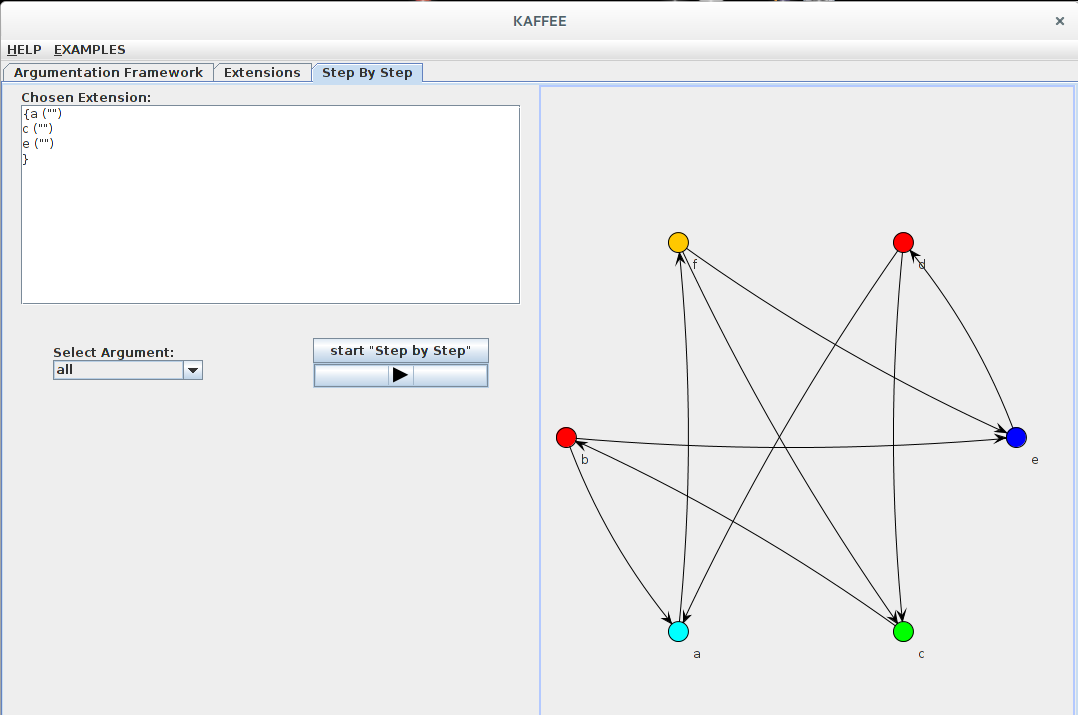
\includegraphics[scale=0.35]{Images/Screenshot_KAFFEE_Tab3.png}
	\end{center}
\caption{Tab "Step By Step"}
\end{figure}

\bigskip
There are also a few built-in shortcuts that make the usage of \textbf{KAFFEE} a little easier:
\begin{description}
	\item{\textbf{ALT+h} \dots\dots\dots Help menu}
	\begin{itemize}
		\item{\textbf{ALT+g} \dots link to the gibhub project containing all the sources, code etc}
		\item{\textbf{ALT+c} \dots feel free to email me}
	\end{itemize}
	\item{\textbf{ALT+e} \dots\dots\dots Examples menu}
	\begin{itemize}
		\item{\textbf{ALT+2} \dots import example \ref{s1 s2 b1 b2 ex}}
		\item{\textbf{ALT+3} \dots import example \ref{s1 s2 ex}}
		\item{\textbf{ALT+4} \dots import example \ref{b loop ex}}
		\item{\textbf{ALT+s} \dots import example "Step By Step"}
	\end{itemize}
\end{description}


%references
\printbibliography

\end{document}
